\chapter{Methodology}
\section{System Model \& Environment}
The proposed network architecture in use for this problem consists of a \acrshort{uav}-\acrshort{bs} for providing network coverage to a set of legitimate \acrshort{gu}s, in which physical layer security is upheld with the use of an \acrshort{ans} to mask the wireless signal from eavesdroppers attempting to perform \acrshort{mitm} attacks on legitimate communications links. 
A diagrammatic representation of the system architecture is shown in Fig. \ref{fig:mengsc_simplified_architecture}, with eavesdroppers referred to as "Eves" and the \acrshort{uav}-\acrshort{bs} shown to provide network coverage for a set of $\mathcal{K}$ legitimate \acrshort{gu}s.
\begin{figure}[ht!]
    \centering
    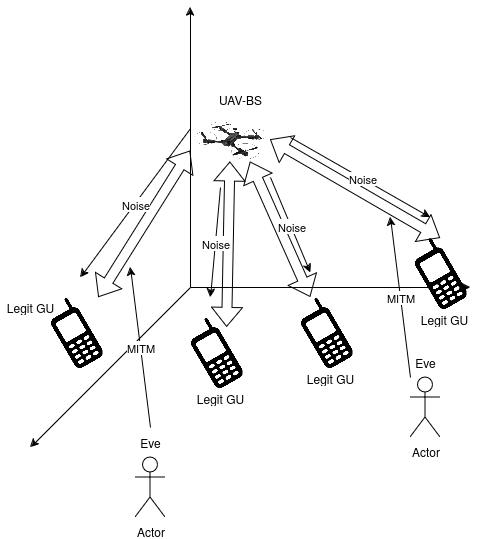
\includegraphics[width=0.7\textwidth]{figures/MEngSc_Thesis_system_architecture_updated.drawio.png}
    \caption{Simplified Diagram of the System Architecture}
    \label{fig:mengsc_simplified_architecture}
\end{figure}

Within the system architecture, there is a set $\mathcal{K}$ of K legitimate \acrshort{gu}s, a set $\mathcal{M}$ of E Eves and a set $\mathcal{X}$ of X \acrshort{uav}-\acrshort{bs}s. 
\subsection{\texorpdfstring{\acrshort{uav}-\acrshort{bs}}{UAV-BS}}
The purpose of the \acrshort{uav}-\acrshort{bs}s are to establish and maintain \acrshort{uav}-\acrshort{gu} communication links with legitimate \acrshort{gu}s while ensuring those communications are physically secure and maintaining an acceptable secrecy rate.  
They provide network coverage to the \acrshort{lu}s and their trajectory, data rate of exchange, energy efficiency and secrecy rate must be optimised to ensure the delivery of adequately secure and energy-efficient communication links for legitimate \acrshort{gu}s. 
The mobility model for the \acrshort{uav} is shown in \ref{eq:uav_mobility_model} \cite{silvirianti_layerwise_2024}. 
\begin{equation} \label{eq:uav_mobility_model}
   v_{\acrshort{uav}} (t) = \delta V_{max}, \ 0 < \delta \le 1
\end{equation}
In this model, the \acrshort{uav}-\acrshort{bs}s can only be connected to the legitimate \acrshort{gu}s and must generate an \acrshort{ans} to combat eavesdropping from Eves based on their observed positions. 
\subsection{Legitimate \texorpdfstring{\acrshort{gu}s}{GUs}}
The \acrshort{lu}s within the system model are the \acrshort{gu}s that the \acrshort{uav}-\acrshort{bs} wishes to communicate with secrectly. 
This involves the \acrshort{lu} having to receive a noisy signal that contains the desired modulated data for the \acrshort{lu} with an \acrshort{ans} that the \acrshort{lu} is provided with information about to enable the \acrshort{lu}'s receiver to filter the \acrshort{ans} from the signal. 
\subsection{Eavesdroppers}
The Eves within the system are eavesdroppers that wish to perform \acrshort{mitm} attacks by detecting and storing the \acrshort{uav}-\acrshort{lu} communications data. 
With the Eves in the environment, they have an eavesdropping rate $R_{E, k} (t), \forall \ k$ for each of the K \acrshort{lu}s which describes how much data they are managing to intercept and store between the \acrshort{uav}-\acrshort{bs} and any of the \acrshort{lu}s. 
The \acrshort{uav}-\acrshort{bs} must estimate the worst-possible value for $R_{E, k} (t)$ to inject \acrshort{ans} into the modulated waveform that minimises the \acrshort{snr} for all E $\in \mathcal{M}$ Eves. 
\subsection{\texorpdfstring{\acrshort{noma}}{NOMA} Communications Model}
A \acrshort{noma} communication scheme has been chosen as it offers potentially higher data exchange rates and all \acrshort{gu}s can be communicated with by the \acrshort{uav}-\acrshort{bs} using a \acrshort{mimo} antenna array on the \acrshort{uav} without the need for division of frequency or time for multiple \acrshort{gu}s to communicate with the \acrshort{uav}. 
The transmitted signal using \acrshort{noma} is shown in \ref{eq:tx_signal_noma} and the received signal is shown in \ref{eq:rx_signal_noma} \cite{silvirianti_layerwise_2024, bizaki_towards_2016}. 
\begin{equation} \label{eq:tx_signal_noma}
    x_{n} = \sum_{k=1}^{K} \sqrt{P_{k, n}^{Tx}} s_{k}
\end{equation}
\begin{equation} \label{eq:rx_signal_noma}
   y_{n} = h_{k, n} (t) x_{n} + I_{k, n}
\end{equation}
In \ref{eq:tx_signal_noma}, $P_{k, n}^{Tx}$ refers to the transmitted signal power and $s_k$ refers to the modulated symbols being transmitted. 
In \ref{eq:rx_signal_noma}, $h_{k, n}$ is the channel gain and $I_{k, n}$ is the interference in the channel caused by the other \acrshort{gu}s being communicated to be the \acrshort{uav}-\acrshort{bs}. 
$I_{k, n}$ in \ref{eq:rx_signal_noma} is removed from the received signal with the use of \acrfull{sic}. 

\subsection{Rician Channel Model \& Environmental Considerations}
The Rician channel model describes a communications channel in which the propagating waveform is made up of a dominant \acrshort{los} path between the receiver and transmitter as well as non-dominant paths. 
The channel model can be characterised with the use of Rician K-factors and $\Omega$-factors \cite{rice_statistical_1948}, shown in \ref{eq:rician_k_factor} and \ref{eq:rician_omega_factor}. 
Rician K-factors describe the ratio of the dominant signal power to the non-dominant signal power in a communication channel. 
The $\Omega$-factors act as a scaling factor for the Rician distribution and is the sum of the dominant and scattered paths. 
%\begin{equation} \label{eq:cosine_wave}
%    s(t) = cos(\omega_{c}t)
%\end{equation}
\begin{equation} \label{eq:dom_and_non_dom_signal}
    v(t) = C \cdot cos(\omega_{c}t) + \sum_{n=1}^{N} r_n cos(\omega_{c}t + f_n)
\end{equation}
\begin{equation} \label{eq:rician_k_factor}
    K = \frac{v^{2}}{2\sigma^{2}}
\end{equation}
\begin{equation} \label{eq:rician_omega_factor}
    \Omega = v^{2} + 2\sigma^{2}
\end{equation} 

The K-factors are computed dynamically with the use of channel gain coefficients that are fixed parameters of the channel, $A_{1}$ and $A_{2}$. 
The elevation angle, $\theta$ between the \acrshort{uav}-\acrshort{bs} and a given \acrshort{gu} is given by \ref{eq:rician_theta} \cite{you_3d_2019}.
\begin{equation} \label{eq:rician_theta}
   \theta = \sin^{-1}\begin{pmatrix}
       \frac{z_{U}}{d_{U}} 
   \end{pmatrix}
\end{equation}
\begin{equation} \label{eq:dynamic_k_factor}
    K = A_{1} e^{A_{2} \theta}
\end{equation}
\begin{equation} \label{eq:rician_g_val}
    g_{U}[k] = \sqrt{\frac{K}{1+K}} g + \sqrt{\frac{1}{K+1}} \tilde{g}
\end{equation}
\begin{equation} \label{eq:pathloss_equation}
   \zeta_{k, n}^{fs} = 20\log_{10}(d_{U} [k]) + 20\log_{10}(f_{c}) + 20\log_{10} \begin{pmatrix}
       \frac{4\pi}{c}
   \end{pmatrix}
\end{equation}
\begin{equation} \label{eq:dynamic_rician_gain}
   h_{U} [k] = g_{U} [k] d_{U} [k]^{-\zeta_{k, n}}
\end{equation}
In \ref{eq:rician_g_val}, $g$ is the deterministic \acrshort{los} component and $\tilde{g}$ is the \acrfull{nlos} random scattered components, which is represented as a \acrfull{cscg}. 
The \acrfull{fspl} exponent shown in \ref{eq:pathloss_equation} in dB, $\zeta_{k, n}$ and $f_{c}$ refers to the carrier frequency of the waveform and $c$ refers to the speed of light. 
The channel gain $h_{U} [k]$ shown in \ref{eq:dynamic_rician_gain} is a function of \ref{eq:rician_g_val}, \ref{eq:pathloss_equation} and $d_{U} [k]$ \cite{li_joint_2024}. 

\section{Mathematical Derivations \& Problem Definition}
The desired outcome of the algorithm and overall system involving \acrshort{uav}s as networking platforms is that the \acrshort{uav}s acting in the environment can perform their task of providing optimal network coverage that must be energy efficient, secret and secure for legitimate \acrshort{gu}s while also ensuring that eavesdropping \acrshort{gu}s are prevented from eavesdropping on legitimate \acrshort{uav}-\acrshort{gu} communications. 
The maximisation of the secrecy rate is a joint optimisation problem that is reliant on the maximisation of the energy efficiency, the maximisation of the data exchange rate, the optimisation of the data exchange rate and the minimisation of the \acrshort{uav} trajectory. The definitions and explanations for these optimisation problems are outlined in the following subsections. 
\subsection{Secrecy Rate Optimisation}
The secrecy rate optimisation is derived from the \acrshort{noma} data exchange rate optimisation, energy efficiency optimisation and the \acrshort{uav} trajectory optimisation. 

The secrecy rate, with aspects adapted from \cite{zhang_one_2025}, with the model for \acrshort{noma} communications from \cite{silvirianti_layerwise_2024}, is derived from the subchannel bandwidth, which allocates a frequency band from the total carrier frequency bandwidth at a given time in which a portion of the total transmit power is allocated to each \acrshort{gu} based on each of their respective channel gains, $h_{U, k}$.
\begin{equation} \label{eq:noma_subchannel_bw}
   \sum_{k=1}^{K} B_{sc} \le BW_{f_{c}}
\end{equation}
As shown in \ref{eq:noma_subchannel_bw}, the sum of the subchannel bandwidths must not exceed the total bandwidth of the carrier frequency $f_{c}$. 

The position of the \acrshort{uav} must only change such that it cannot exceed the maximum step change, $\delta$ multiplied by the maximum velocity of the \acrshort{uav}, $V_{max}$. 

Equation \ref{eq:uav_power_constraint} shows the allocated transmit power cannot exceed the maximum allocated power in timeslot $n$. 
\begin{equation} \label{eq:uav_power_constraint}
    \sum_{i=0}^{I} P_{U, i} [n] \le P_{U, k}^{Tx} [n], \forall n
\end{equation}
The distance between the \acrshort{uav} and \acrshort{gu}, shown in \ref{eq:distance_uav_gu} is factored into the channel gain along with the directional gain of the antennae on the \acrshort{uav} and the \acrshort{gu}. 
This \acrshort{uav} channel gain $h_{U, k}$ for $k$ \acrshort{gu}s, shown in \ref{eq:channel_gain_uav_gu} is subsequently used in \ref{eq:snr_uav_gu} for computing the data rate in the \acrshort{uav}-\acrshort{gu} communications channel, which in turn, is used to compute the \acrshort{masr} or the secrecy rate of the communications. 

\begin{equation} \label{eq:distance_uav_gu}
    d_{U, k} = \sqrt{(x_{U, k}-x_{GU, k})^2 + (y_{U, k}-y_{GU, k})^2 + (z_{U, k}-z_{GU, k})^2}
\end{equation}
\begin{equation} \label{eq:channel_gain_uav_gu}
    h_{U, k} [n] = g_{U, k} [n] d_{U, k} [n]^{-\zeta_{k, n}}
    %h_{U, k} = \frac{G_{0}G_{1}\beta_{0}}{(d_{U, k}[n])^2}
\end{equation} 
\begin{equation} \label{eq:snr_uav_gu}
    \acrshort{snr}: \gamma_{U, k, i} [n] = \frac{P_{U, i}[n] h_{U, k}[n]}{I_{k, n} + (\sigma_{\acrshort{los}} + \sigma_{\acrshort{nlos}} + \sigma_{\acrshort{awgn}})^{2}}
    %\acrshort{snr}: \gamma_{U, k, i} [n] = \frac{P_{U, i}[n] h_{U, k}[n]}{B_{0}N_{0}^{GU}}
\end{equation} 
The \acrshort{snr} is the ratio of the channel power by the channel gain to the sum of the \acrshort{awgn}, \acrshort{los} and \acrshort{nlos} noise power values and $I_k, n$ is the interference from other users, which is canclled with \acrshort{sic}. 
The rate of data exchange in the \acrshort{uav}-\acrshort{gu} communication link is expressed in \ref{eq:uav_gu_data_rate}, which is a function of the subchannel bandwidth $B_{sc} [n]$ in slot $[n]$ and the \acrshort{snr}. 
\begin{equation} \label{eq:uav_gu_data_rate}
    R_{U, m, i} [n] = B_{sc}[n] \log_{2} (1 + \gamma_{U, m, i}[n]), \forall i, m, n
\end{equation} 
The position of Eve $m$ in timeslot $n$ is shown in \ref{eq:exact_eve_position}. 
\begin{equation} \label{eq:exact_eve_position}
    s_{m} [n] = \begin{pmatrix}
        x_{m} [n] & y_{m} [n] & z_{m} [n]
    \end{pmatrix} ^{T}
\end{equation}
The \acrshort{uav}-\acrshort{bs} observes the state with all of the \acrshort{gu}s, and those that have not been authenticated as \acrshort{lu}s within the network are classed as Eves. 
Based on the proximity of the perceived Eves within the environment, the \acrshort{uav}-\acrshort{bs} must calculate the eavesdropping rate that each Eve has for each \acrshort{lu} as shown in \ref{eq:eavesdropping_rate_eq}. 
\begin{equation} \label{eq:eavesdropping_rate_eq}
   R_{E, k, m} [n] = B_{sc} [n] \log_{2} (1 + \gamma_{E, k, n} [n]), \forall \ k, m, n
\end{equation}
The eavesdropping rates with the highest values are used for the calculation of the \acrshort{ans}. 
With this secrecy scheme, each of the \acrshort{lu}s are protected from the worst-case eavesdropping rate, i.e., the eavesdropping rate of whichever Eve has the greatest \acrshort{snr} to conduct their \acrshort{mitm} attack. 
%The estimated position of Eve $m$ is $\tilde{s}_{m}$, which is a circle of radius $\mathcal{E}$ with estimation errors $\Delta x_{m} [n], \Delta y_{m} [n] \in \mathcal{E}$. 
%The relationship between the exact and estimated Eve position is shown in \ref{eq:estimated_eve_position_x} and \ref{eq:estimated_eve_position_y}. 
%\begin{equation} \label{eq:estimated_eve_position_x}
%    x_{m} [n] = \tilde{x}_{m} [n] + \Delta x_{m} [n]
%\end{equation}
%\begin{equation} \label{eq:estimated_eve_position_y}
%    y_{m} [n] = \tilde{y}_{m} [n] + \Delta y_{m} [n]
%\end{equation}
%The actual Eve position is within a circle of radius $\tilde{s}_{m} [n]$ with a radius of $\mathcal{E}$ such that $\mathcal{E} \le ||q_{U}[n] - \tilde{s}_{m} [n]||$. 
The worst-case eavesdropping rate is shown in \ref{eq:worst_case_eve_rate} and the minimum secrecy rate is expressed in \ref{eq:secrecy_rate}, being the absolute difference between \ref{eq:uav_gu_data_rate} and \ref{eq:worst_case_eve_rate} \cite{zhang_one_2025}. 
The secrecy sum rate is expressed in \ref{eq:secrecy_sum_rate}
%\begin{equation}\label{eq:worst_case_eve_rate}
%    \Phi = \underset{\mathcal{M}}{\max}\begin{Bmatrix} \underset{\Delta x_{m} [n], \Delta y_{m} [n] \in X}{\max} 
%        R_{E, k, m}[n]
%    \end{Bmatrix}, \forall k, m, n
%\end{equation} 
\begin{equation}\label{eq:worst_case_eve_rate}
    \Phi = \underset{\mathcal{M}}{\max}\begin{Bmatrix} \underset{\max \gamma_{E, k, m}[n]}{\max} 
        R_{E, k, m}[n]
    \end{Bmatrix}, \forall k, m, n
\end{equation} 
\begin{equation} \label{eq:secrecy_rate}
    R_{k, i}^{sec} [n] = [R_{U, k, i} [n] - \Phi]^{+}, \forall i, k, n
\end{equation} 
\begin{equation} \label{eq:secrecy_sum_rate}
    \bar{R}_{k, i}^{sec} [n] = \frac{1}{N} \sum_{n=1}^{N} \sum_{i=1}^{I} R_{k, i}^{sec} [n], \forall k
\end{equation}
%\hl{REWRITE THIS PORTION WITH PROPER EQUATION REFERENCING FOR THE CONSTRAINTS AND OBJECTIVE FUNCTION} 

The secrecy rate is to be maximised subject to the following constraints, the \acrshort{uav} must not exceed its range and altitude limits in three-dimensional Cartesian space (\ref{eq:secrecy_rate_position_constraint}), the power consumption must not exceed the maximum power consumption over time (\ref{eq:secrecy_rate_power_constraint}), the allocated transmit power must be greater than or equal to 0 (\ref{eq:secrecy_rate_tx_power_constraint}) and the change in position of the \acrshort{uav} must not exceed the step size $\delta$ multiplied by the maximum velocity of the \acrshort{uav}, $V_{max}$ (\ref{eq:secrecy_rate_trajectory_constraint}). 
The co-ordinate position of the \acrshort{uav} in Cartesian co-ordinates, $[x_{U}, y_{U}, z_{U}]$ is denoted as $q_{U}$ in \ref{eq:secrecy_rate_trajectory_constraint}.
\begin{equation} \label{eq:secrecy_rate_objective_function}
    \underset{q_{U}, A, E, Q}{\max}\bar{R}_{k, i}^{sec}, s.t.
\end{equation} 
\begin{equation} \label{eq:secrecy_rate_power_constraint}
    \sum_{i=1}^{I} P_{U, i} \le P_{tot}
\end{equation}
\begin{equation} \label{eq:secrecy_rate_tx_power_constraint}
    0 \le P_{U, k}^{Tx} \le P_{U_{tot}}^{Tx}, \forall k
\end{equation}
\begin{equation} \label{eq:secrecy_rate_subchannel_constraint}
    \sum_{k=1}^{K} B_{sc, k} [n] \le BW_{f_c}, \forall \ k
\end{equation}
\begin{equation} \label{eq:secrecy_rate_e_cons_constraint}
    E_{cons} \le E_{max}
\end{equation} 
\begin{equation} \label{eq:secrecy_rate_trajectory_constraint}
    ||q_{U}[n+1] - q_{U}[n]||^2 \le (\delta V_{max})^2, \forall \ n
\end{equation} 
\begin{equation} \label{eq:secrecy_rate_position_constraint}
    x_{min} \le x_{U} \le x_{max}
    ,\  
    y_{min} \le y_{U} \le y_{max}
    ,\  
    z_{min} \le z_{U} \le z_{max}
\end{equation}
The subchannel allocation, \acrshort{uav} trajectory and energy efficiency must be maximised as part of this joint optimisation problem to ensure that the secrecy rate is maximised. 
The Eve \acrshort{snr} must also be minimised in order to minimise the eavesdropping rate, as described in \ref{eq:maximise_eve_snr_constraint} and \ref{eq:minimise_eve_rate_constraint}. 
The maximisation of the \acrshort{uav}-\acrshort{lu} data rate is also required to minimise the eavesdropping rate and the maximisation of the \acrshort{ans}, $\psi$. 
\begin{equation} \label{eq:maximise_eve_snr_constraint}
   \underset{\psi}{\max}\gamma_{E, m, k}
\end{equation}
\begin{equation} \label{eq:minimise_eve_rate_constraint}
   \underset{\min \gamma_{E, k, m}}{\min} R_{E, k, m} [n], \forall \ k, m, n
\end{equation}
\subsection{Energy Efficiency Optimisation}
The energy consumption mathematical model has been adapted from \cite{silvirianti_layerwise_2024} to describe the consumption of energy on board any given \acrshort{uav}. The model accounts for the energy consumed while travelling, hovering, by the avionics and the communication energy. 
The energy consumption at time $t$, $E_{cons}(t)$ can be expressed as shown in \ref{eq:energy_cons_model}.

%\hl{CHANGE THE MASS CALCULATION AS IT SHOULD BE A CONSTANT. NO CLEAR REASON TO SUM IT TWICE}
\begin{equation} \label{eq:energy_cons_model}
    E_{cons}(t) = \sum_{n=1}^{N} \sum_{k=1}^{K_n} \left (\underbrace{\frac{\sum_{i=1}^{I} n_{i} g |q_{U}(t)|}{K\textit{r}}}_{\text{Travelling}} + 
    \underbrace{\frac{((\sum_{i=1}^{I}n_i)g)^{\frac{3}{2}}}{\sqrt{2 r \zeta \theta}}}_{\text{Hovering}} +
    \underbrace{\Lambda \frac{|q_{U}(t)|}{v(t)}}_{\text{Avionics}} + 
    \underbrace{P_{k, n}^{Tx}(t) R_{k, n}(t)}_{\text{Communications}} \right)
\end{equation}
In \ref{eq:energy_cons_model}, $n_{i}$ is the mass of the \acrshort{uav} frame and battery, $g$ is acceleration due to gravity ($9.81\ m s^{-2}$), $q_{U}(t)$ is the position of the \acrshort{uav} at time $t$, $K$ is the lift-to-drag ratio, shown in \ref{eq:lift_to_drag_ratio}, $r$ denotes the number of \acrshort{uav} rotors, $\zeta$ refers to the air density, $\theta$ is the spinning blade of a single rotor, $\Lambda$ is the avionics power and $v(t)$ is the velocity of the \acrshort{uav} at time $t$ \cite{silvirianti_layerwise_2024, zhang_energy_2021}. 

%\hl{POSSIBLE NEED TO UPDATE LIFT TO DRAG RATIO HERE FOR QUADCOPTER UAV}
\begin{equation} \label{eq:lift_to_drag_ratio}
   K = \frac{L}{D} = \frac{\sum_{i=1}^2 n_{i} g v_{U}}{P}
\end{equation}
$\sum_{i=1}^2 n_{i}$ is the mass of the \acrshort{uav} frame and battery, $g$ is the acceleration due to gravity, $v_{U}$ is the velocity of the \acrshort{uav} and $P$ is the power required for the \acrshort{uav} \cite{theys_forward_2020}. 
%\begin{equation} \label{eq:lift_to_drag_ratio}
%    K = \left (\frac{L}{D} \right )_{max} = \frac{1}{2} \sqrt{\frac{\pi \epsilon (AR)}{C_{D, 0}}}
%\end{equation}
%Where $\epsilon$ is the span efficiency factor, $AR$ refers to the aspect ratio of the \acrshort{uav} wings and $C_{D, 0}$ is the zero-lift drag coefficient. \hl{CITATION}

As can be seen in the expression for the communications energy, the transmit power is included within the energy consumption model, which is factored into the secrecy rate in \ref{eq:secrecy_rate_objective_function}.
The total energy efficiency can be expressed as shown in \ref{eq:energy_efficiency}. 
\begin{equation} \label{eq:energy_efficiency}
    \eta (T) = \int_{t=1}^{T} \frac{\sum_{n=1}^{N} \sum_{k=1}^{K_{n}} R_{k, n}(t)}{E_{cons}(t)} dt
\end{equation}
The energy efficiency must be maximised as part of the joint optimisation expressed in \ref{eq:secrecy_rate_objective_function}. The optimisation of \ref{eq:energy_efficiency} is detailed in \ref{eq:energy_efficiency_objective_function} and the maximisation of $\eta(t)$ involves the optimisation of the user grouping, \acrshort{uav} position and power allocation on the \acrshort{uav}. 
\begin{equation} \label{eq:energy_efficiency_objective_function}
    \underset{G_{n} \in N, q_{U}(t), P_{k, n}^{Tx}(t)}{\max} \eta (t), s.t.
\end{equation}
\begin{equation} \label{eq:energy_efficiency_transmit_power_constraint}
    \sum_{n=1}^{N} \sum_{k=1}^{K_n} P_{k, n}^{Tx} \le P_{UAV}^{Tx} 
\end{equation}
\begin{equation} \label{eq:energy_efficiency_power_coefficient_constraint}
    0 < \sum_{k=1}^{K_n} a_{k, n} \le 1
\end{equation}
\begin{equation} \label{eq:energy_efficiency_power_coefficient_order_constraint}
    a_{1, n} < \dots < a_{K_n, n}
\end{equation}
\begin{equation} \label{eq:energy_efficiency_transmit_rate_coefficient}
    R_{k, n} [n] \ge R_{min}
\end{equation}
\begin{equation} \label{eq:energy_efficiency_position_constraint}
    x_{min} \le x_{U} \le x_{max},\ y_{min} \le y_{U} \le y_{max},\ z_{min} \le z_{U} \le z_{max}
\end{equation}
The constraints applied to \ref{eq:energy_efficiency_objective_function} include the limit of the maximum transmit power in a \acrshort{noma} group of \acrshort{gu}s (\ref{eq:energy_efficiency_transmit_power_constraint}), the transmit power coefficient range for each \acrshort{gu} (\ref{eq:energy_efficiency_power_coefficient_constraint}), the fact that each transmit power coefficient must be ordered such that a higher coefficient is granted to users with a lower channel gain (\ref{eq:energy_efficiency_power_coefficient_order_constraint}), the transmitted data rate must exceed the minimum threshold data rate (\ref{eq:energy_efficiency_transmit_rate_coefficient}) and the \acrshort{uav} must remain within the bounds of its range and altitude (\ref{eq:energy_efficiency_position_constraint}). 

%\subsection{\acrshort{ofdm} Channel Subcarrier Allocation Optimisation}
%\hl{CHANGE THIS TO NOMA DATA RATE OPTIMISATION AS NOMA IS BEING USED IN THE MODEL}
%
%The \acrshort{ofdm} subcarrier channels are a resource for the \acrshort{uav}-\acrshort{bs} to allocate for a given legitimate \acrshort{gu} and they are scheduled such that the subcarrier channel allocation is fair for all \acrshort{gu}s and provides a reasonable \acrfull{qos}. 
%\acrshort{ofdm} is in use due to its high spectral efficiency and resilience to noisy channels. 
%Each subcarrier can be described as shown in \ref{eq:ofdm_subcarrier_wave}. 
%\begin{equation} \label{eq:ofdm_subcarrier_wave}
%    s_{c}(t) = A_{c} e^{j|\omega_{c} + \phi_{c}(t)|}
%\end{equation}
%Where $A_{c}$ is the symbol of the carrier and its magnitude, while $s_{c}(t)$ is a complex wave containing both a magnitude and phase. 
\subsection{Optimisation of \texorpdfstring{\acrshort{uav}-\acrshort{gu}}{UAV-GU} Data Exchange Rate}
As the function of data rate exchange shown in \ref{eq:uav_gu_data_rate} is a function of the \acrshort{snr}, which itself is a function of the channel gain, which is dependent on the distance between the \acrshort{uav}-\acrshort{bs} and any given \acrshort{gu} as a result of the \acrshort{fspl}, the \acrshort{uav}-\acrshort{gu} data exchange rate can be optimised by minimising the distance between the \acrshort{uav}-\acrshort{bs} and all $K$ \acrshort{gu}s. 
To achieve \ref{eq:data_rate_objective_function}, the difference in distances between all \acrshort{gu} to the \acrshort{uav}-\acrshort{bs} must be minimised and the distance between the \acrshort{uav}-\acrshort{bs} to the \acrshort{gu} centroid must be minimised. 
The differences in distances between the \acrshort{uav}-\acrshort{bs} and the \acrshort{gu}s is expressed in \ref{eq:gu_dist_diffs}. 
Minimising this distance as shown in \ref{eq:min_gu_dist_diffs} ensures that all \acrshort{gu}s are receiving a level of network coverage that is above $R_{min}$.
Minimising the distance between the \acrshort{uav}-\acrshort{bs} helps to ensure that the \acrshort{uav} trajectory is optimised, as shown in \ref{eq:uav_trajectory_objective_function}, while also maximising $R_{U, k} [n]$, as expressed in \ref{eq:data_rate_objective_function}. 
The \acrshort{gu} centroid, $C_{GU} [n]$ is the average value between all of the \acrshort{gu} positions. 
\begin{equation} \label{eq:data_rate_objective_function}
    \max R_{U, k} [n]
\end{equation}
\begin{equation} \label{eq:gu_dist_diffs}
    \lambda_{GU} [n] = \sum_{k=1}^{K} \sum_{j \neq k}^{K} |d_{U, k} [n] - d_{U, j}[n]|
\end{equation}
\begin{equation} \label{eq:min_gu_dist_diffs}
    \min \lambda_{GU} [n]
\end{equation}
\begin{equation} \label{eq:gu_centroid}
    C_{GU} [n] = \frac{1}{K} \sum_{k=1}^{K} d_{U, k} [n] + z_{min}
\end{equation}
\begin{equation} \label{eq:min_gu_centroid}
    \min C_{GU} [n]
\end{equation}
The objective functions shown in \ref{eq:data_rate_objective_function}, \ref{eq:min_gu_dist_diffs} and \ref{eq:min_gu_centroid} are subject to the constraints shown in \ref{eq:secrecy_rate_trajectory_constraint}, \ref{eq:secrecy_rate_position_constraint}, \ref{eq:energy_efficiency_transmit_power_constraint} and \ref{eq:energy_efficiency_transmit_rate_coefficient}.  

\subsection{Optimisation of \texorpdfstring{\acrshort{uav}}{UAV} Trajectory}
The \acrshort{uav} trajectory can be expressed as \ref{eq:uav_trajectory}.
\begin{equation} \label{eq:uav_trajectory}
   c(t) = q_{U}[n+1] - q_{U}[n]
\end{equation}
The trajectory is to be minimised such that the \acrshort{uav} can take the shortest path to serve its role for a set of $K$ \acrshort{gu}s and other \acrshort{uav}s. 
\begin{equation} \label{eq:uav_trajectory_objective_function}
   \underset{}{\min}\ q_{U}(t), s.t.
\end{equation}
\begin{equation}\label{eq:traj_boundary_constraints}
    x_{min} \le x_{U} \le x_{max},\ y_{min} \le y_{U} \le y_{max},\ z_{min} \le z_{U} \le z_{max}
\end{equation}
\begin{equation} \label{eq:distance_constraint}
    d_{U}, k \le 100, \forall k
\end{equation}
\section{Algorithms \& System Design}
%\hl{TODO: UPDATE THIS TO REFLECT THAT ONLY ONE UAV-BS WILL BE IN USE (AT LEAST AT PRESENT)}
The proposed approach for solving the outlined optimisation problem leverages \acrshort{drl} to determine the optimal secrecy rate for \acrshort{uav}-\acrshort{gu} communications such that $R_{U, k, n} \forall k, n$ over \acrshort{noma} is optimised, the energy efficiency converges to higher values, the resource allocation is optimised and the \acrshort{uav} trajectories are optimised. 
%A \acrshort{ppo}-based algorithm is used for this problem and solved in the classical computation case and a subsequent implementation of this algorithm, where part of the computation is offloaded to a gate-based quantum computer is also outlined. 
\subsection{Design}
The overall architecture of the system is illustrated in Fig. \ref{fig:system_block_diagram}. 

\begin{figure} [ht!]
    \centering
    %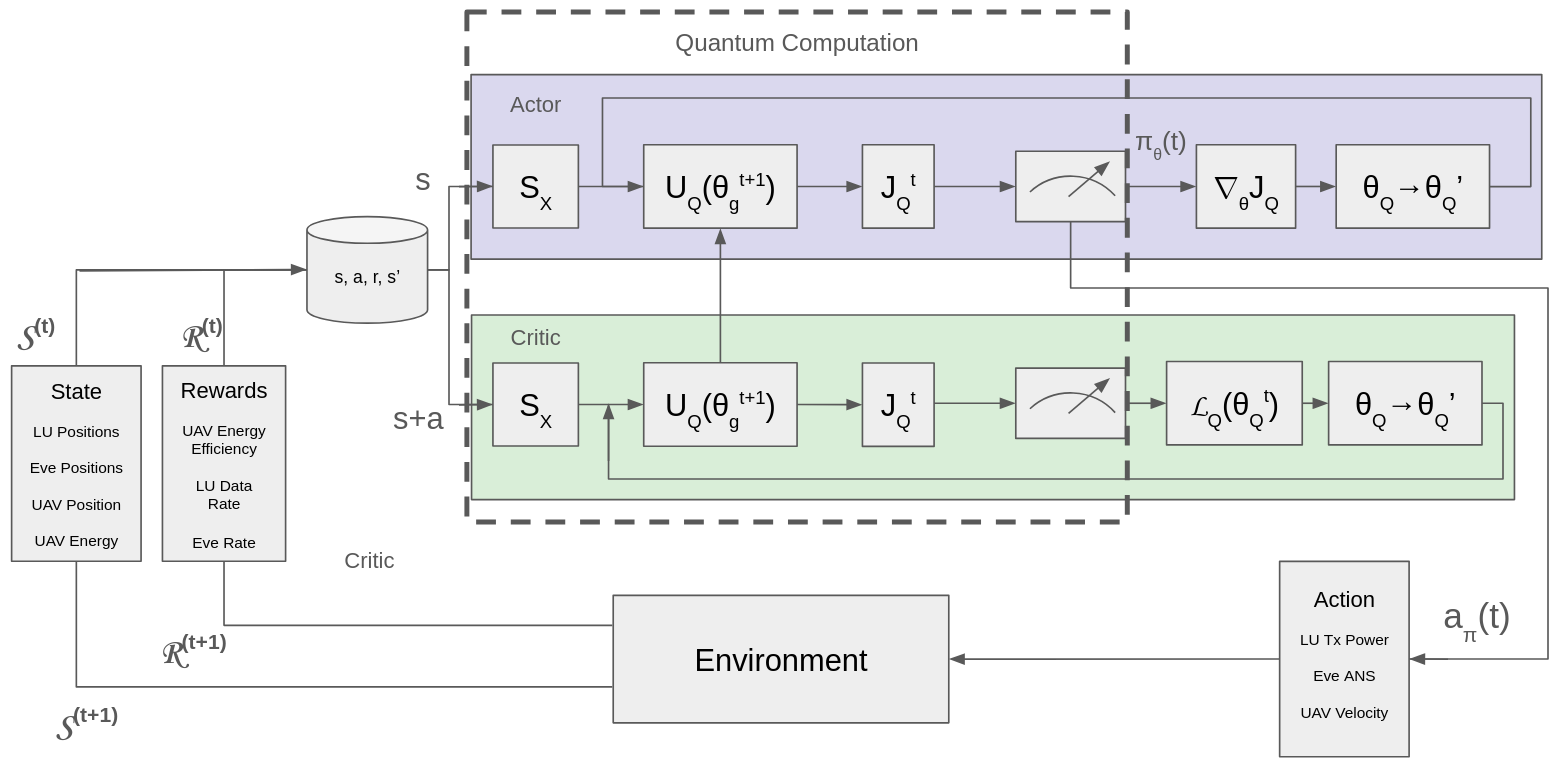
\includegraphics[width=1\textwidth]{figures/annotated_system_block_diagram.png}
    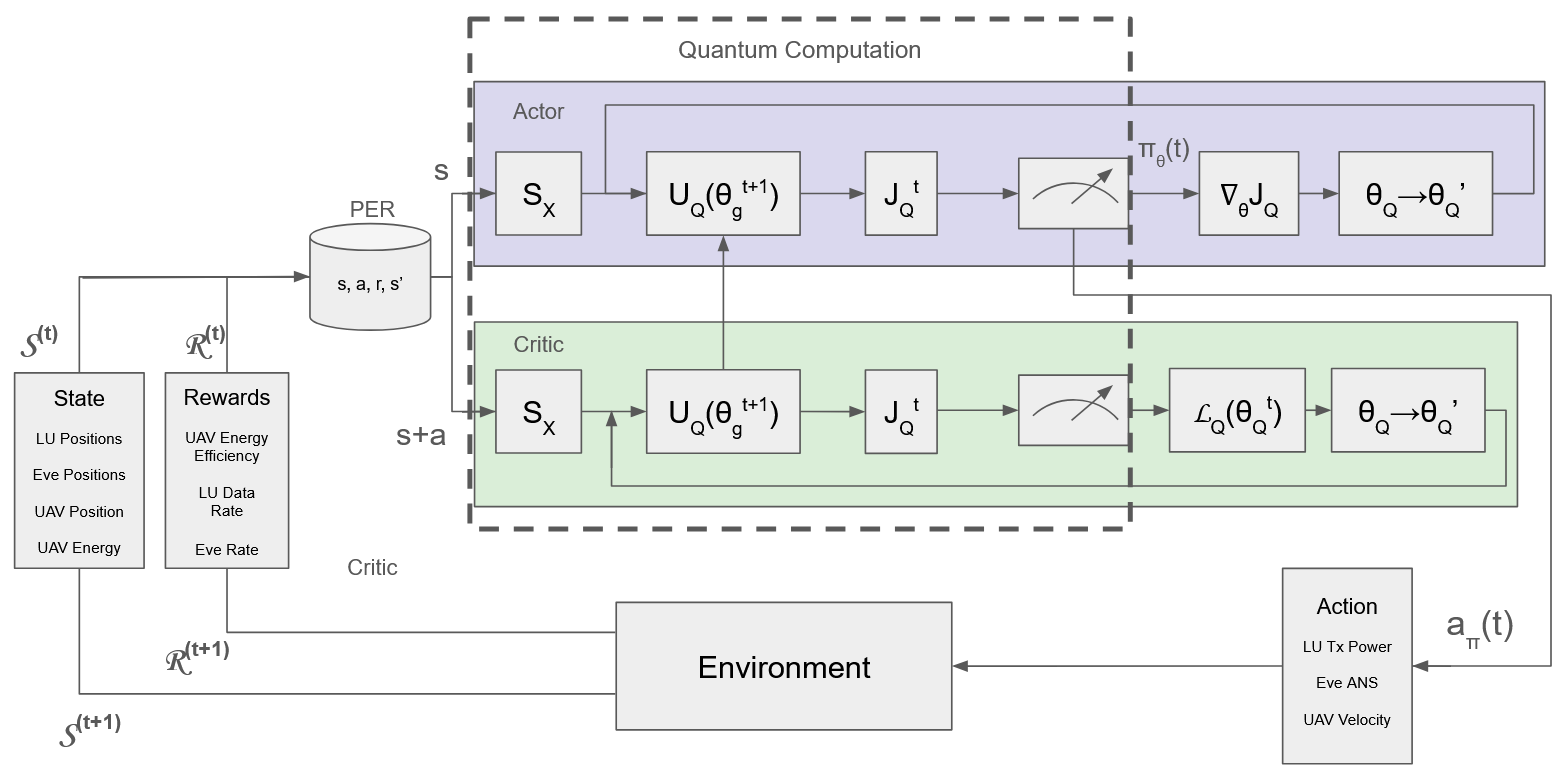
\includegraphics[width=1\textwidth]{figures/system_block_diagram_labelled.png}
    \caption{System Block Diagram}
    \label{fig:system_block_diagram}
\end{figure}
As shown in Fig. \ref{fig:system_block_diagram}, the overall system is a quantum-classical hybrid approach to the joint optimisation problem outlined in the previous section of this chapter. 
This system architecture has been adapted from \cite{silvirianti_layerwise_2024} and \cite{silvirianti_uav_2024}.
The design of the \acrshort{lqdrl} algorithm employing layerwise quantum embedding involves the use of storing parameters of the system as quantum states using a quantum circuit, referred to as an ansatz. 
This process is referred to as quantum encoding. 
The input parameter data is stored in a vector $\textbf{x}$ of $N$ elements, which are encoded into a set of quantum states $\ket{\phi}_{0, 1, \dots, N-1}$. 
The encoding process is denoted as $S_{\textbf{x}}$. 
The \acrshort{uav} is an agent interacting with the environment to observe the state space $s$, determine an action $a$ that is best in line with the desired policy $\pi$ that yields a reward $r$ and creates the updated state space $s'$. 
These parameters are embedded within the ansatz as $N$ qubits, where $N$ denotes the number of parameters required for the quantum data embedding. 
The value function of the selected policy $\pi$ for a state $s$ is shown in \ref{eq:policy_value_function} and $\mu'$ is the learning discount rate \cite{murphy2025reinforcementlearningoverview}. 
\begin{equation} \label{eq:policy_value_function}
   V_{\pi} (s) = E \begin{pmatrix}
       \sum_{t=1}^{T} \mu' r_{t} | s_{0}=s
   \end{pmatrix} 
\end{equation}
The system has been designed as a \acrfull{dqn}. 
Q-learning involves evaluating the quality or value of a state/action pair by determining it's Q-value $Q(s, a)$. 
The Q-value can be updating as shown in \ref{eq:q_value_update} \cite{murphy2025reinforcementlearningoverview}. 
\begin{equation} \label{eq:q_value_update}
   Q^{update} (s, a) = Q^{old} (s, a) + \alpha \begin{pmatrix}
       r_t + \mu \underset{a}{\max} Q (s_{t+1}, a) - Q^{old} (s_{t}, a_{t})
   \end{pmatrix}
\end{equation}
Q-learning is employed to essentially evaluate both \ref{eq:policy_value_function} and the policy itself simultaneously. 
By maximising the Q-value, the quality of state/action pairs can influence the \acrshort{drl} algorithm's agent to perform more optimally as it learns.

The system contains a \acrshort{mer}, which stores the states ($s$), actions ($a$), rewards ($r$) and the next state ($\hat{s}$). 
The experiences of the agent are stored and sampled as the agent learns to optimise it's parameters and actions based on the observed state space which is sampled by the critic to evaluate the quality of an action taken by the actor network. 
The more experiences that the \acrshort{uav} has, the larger it's set of experiences to sample and compare its current action from grows.

\subsection{Quantum Data Embedding \& Parameter Encoding}
The ansatz in use for the actor and critic networks involves the encoding of data into the circuit that is measured and decoded at the output and passed to a gradient descent algorithm that employs the two-term parameter-shift rule to compute the quantum gradients. 
The actor network takes the observed state space at time $t$, which contains $2K+4$ dimensions, where $K\ \in \mathcal{K}$, i.e., the number of \acrshort{gu}s in the environment. 
The critic network takes both the state and action at time $t$ as its inputs, which contains $(2K+4)+5$ dimensions as the action space contains 5 dimensions, the \acrshort{uav} transmit power, the \acrshort{ans}s for the Eves and the \acrshort{uav} velocity and trajectory. 

The quantum gates in use within the quantum circuits are the Hamiltonian, x-rotation gate, y-rotation gate and the controlled Pauli-Z (denoted as CZ) gates, whose matrix representations are shown in \ref{eq:hamiltonian_operator}, \ref{eq:rx_gate_matrix}, \ref{eq:ry_gate_matrix} and \ref{eq:cz_gate_matrix}. 
\begin{equation} \label{eq:hamiltonian_operator}
   H = \begin{pmatrix}
       1 & 1 \\
       1 & -1
   \end{pmatrix} 
\end{equation}
\begin{equation} \label{eq:rx_gate_matrix}
   RX (\theta) = \begin{pmatrix}
       \cos(\frac{\theta}{2}) & -i \cdot \sin(\frac{\theta}{2}) \\
        -i \cdot \sin(\frac{\theta}{2}) & \cos(\frac{\theta}{2})
   \end{pmatrix} 
\end{equation}
\begin{equation} \label{eq:ry_gate_matrix}
   RY (\theta) = \begin{pmatrix}
        cos(\frac{\theta}{2}) & -sin(\frac{\theta}{2}) \\
        sin(\frac{\theta}{2}) & cos(\frac{\theta}{2})
    \end{pmatrix} 
\end{equation}
\begin{equation} \label{eq:cz_gate_matrix}
   CZ = \begin{pmatrix}
       1 & 0 & 0 & 0 \\
       0 & 1 & 0 & 0 \\
       0 & 0 & 1 & 0 \\
       1 & 0 & 0 & -1
   \end{pmatrix} 
\end{equation}

The quantum embedding system design uses the ansatz presented in \cite{silvirianti_layerwise_2024} and the quantum circuit in use for the actor and critic networks is presented in Fig. \ref{fig:single_layer_ansatz}. 

\begin{figure}[ht!]
    \centering
    \begin{quantikz}
        \lstick{$\ket{0}$} & \gate{H} \gategroup[5, steps=1, style={inner sep=1pt}]{Encoding} & \qw & \qw & \gate{RX(\textbf{$x_{1}^{(1)}$})} \gategroup[5, steps=1, style={inner sep=1pt}]{Input Vector} &\qw &\qw & \ctrl{1} \gategroup[5, steps=3, style={inner sep=1pt}]{Entanglement} & \qw & \qw & \qw & \qw & \gate{RY(\textbf{$\theta_{1}^{(1)}$})} \gategroup[5, steps=1, style={inner sep=1pt}]{Gradients} & \qw & \meter[label, style={inner sep=1pt}]{1}{} & \\
        \lstick{$\ket{0}$} & \gate{H} & \qw & \qw & \gate{RX(\textbf{$x_{2}^{(1)}$})} & \qw & \qw & \control{} & \ctrl{1} & \qw & \qw & \qw & \gate{RY(\textbf{$\theta_{2}^{(1)}$})} & \qw & \meter{2}{} & \\
        \vdots & \vdots & \vdots & \vdots & \vdots & \vdots & \vdots & \vdots &\vdots &\vdots &\vdots & \vdots &\vdots &\vdots &\vdots \\
        \lstick{$\ket{0}$} & \gate{H} & \qw & \qw & \gate{RX(\textbf{$x_{N-1}^{(1)}$})} & \qw & \qw & \qw & \ctrl{-1} & \ctrl{1} & \qw & \qw & \gate{RY(\textbf{$\theta_{G-1}^{(1)}$})} & \qw & \meter{N-1}{} & \\
        \lstick{$\ket{0}$} & \gate{H} & \qw & \qw & \gate{RX(\textbf{$x_{N}^{(1)}$})} & \qw & \qw & \qw &  \qw & \control{} & \qw & \qw & \gate{RY(\textbf{$\theta_{G}^{(1)}$})} & \qw & \meter{N}{} & 
    \end{quantikz}
    \caption{Single-Layered Actor-Critic Network Ansatz}
    \label{fig:single_layer_ansatz}
\end{figure}

The actor and critic quantum circuits can be represented as unitary operators, which evolve a Hermitian operator over time. 
The equation describing the ansatz design presented in Fig. \ref{fig:single_layer_ansatz} is shown in \ref{eq:ansatz_unitary} \cite{silvirianti_layerwise_2024}. 
\begin{equation} \label{eq:ansatz_unitary}
    U_{LQ} (\theta) = \bigotimes_{g=1}^{G} \bigotimes_{n=1}^{N} (S_{\theta_{g}}) \begin{pmatrix}
\Pi_{n=1}^{N} CZ(\phi_{2}|\phi_{1}) \otimes \dots \otimes CZ(\phi_{N}|\phi_{N-1})
\end{pmatrix} (S_{\textbf{x}_{n}})H
\end{equation}
The encoding of the input parameter data vector $\textbf{x}$ is shown in \ref{eq:input_vector_encoding} and the encoding of the quantum gradients is shown in \ref{eq:gradient_encoding}. 
\begin{equation} \label{eq:input_vector_encoding}
   S_{\textbf{x}}: \bigotimes_{n=1}^{N} RX \begin{pmatrix}
       \textbf{x}_{n}
   \end{pmatrix}
\end{equation}
\begin{equation} \label{eq:gradient_encoding}
   S_{\theta} : \bigotimes_{g=1}^{G} RY \begin{pmatrix}
       \theta_g
   \end{pmatrix}
\end{equation}
The decoding operation for the actor network is shown in \ref{eq:actor_decoding_expectation_value}, \ref{eq:actor_decoding_op} and the operation is reduced to \ref{eq:actor_decoding}, where $K_{shots}$ is the number of measurements taken of the output \cite{silvirianti_layerwise_2024}. 
\begin{equation} \label{eq:actor_decoding_expectation_value}
   J_{Q} = \braket{0|U_{Q}^{\dagger}(x) H U_{Q}(x)|0}
\end{equation}
\begin{equation} \label{eq:actor_decoding_op}
   J_{Q} (\theta_{g}) = Z(\ket{\phi_{n}})
\end{equation}
\begin{equation} \label{eq:actor_decoding}
    y \xleftarrow[]{} \frac{1}{K_{shots}} \sum_{k=1}^{K_{shots}} Z(\ket{\phi})
\end{equation}
As the actor's output state has to be measured in the computational basis, its basis is transformed into the Pauli Z-basis for measurement. 

The critic outputs the loss calculation based on the generated Q-value for a given action $a$ in state $s$ based on target rewards sampled from the \acrshort{mer}. 
This operation is shown in \ref{eq:critic_decoding_op} \cite{silvirianti_layerwise_2024}. 
\begin{equation} \label{eq:critic_decoding_op}
   \mathcal{L}_{Q} = \frac{1}{N_{data}} \sum_{n=1}^{N_{data}} (y_{n} - \hat{y}_{n})^2
\end{equation}
The variable $y_{n}$ refers to the actor output and $\hat{y}_{n}$ refers to the target output. 
The difference between these values is taken and squared to ensure that the result is positive-valued. 
The critic is calculating a loss value based on the difference between an optimal target action and the action taken by the agent. 

The $\theta$ parameters are updated for each timestep as shown in \ref{eq:theta_parameter_update} \cite{silvirianti_layerwise_2024}.  

\begin{equation} \label{eq:theta_parameter_update}
   \theta_{g} = \theta_{g} - \beta \nabla_{\theta_{g}} \mathcal{L}_{Q} (\theta_{g})
\end{equation}
$\theta_{0}, \theta_{1} \dots \theta_{G-1}, \theta_{G}$ is updated using the gradient descent calculation of \ref{eq:critic_decoding_op} multiplied by $\beta$, which is the learning rate for the critic \cite{silvirianti_layerwise_2024}. 
\subsection{Classical Computation of Gradient Descent}
The two-term parameter shift algorithm is used to compute the gradient descent for computation of new parameters in the quantum circuit after every timestep.  
This approach involves modelling the expectation value of the measured output of a quantum circuit as a Fourier series using a finite set of \acrfull{pud}.
The Fourier series has a finite number of terms and can be computed classically. 
The \acrfull{dft} can be used to determine the coefficients of the Fourier series. 
The expectation value for a general gate $U(x) = e^{ixG}$ defined by a Hermitian operator $G$ and parameterised by $x$ can be expressed as shown in \ref{eq:param_shit_expectation_value}. 
\begin{equation} \label{eq:param_shit_expectation_value}
    E(x) = a_{0} + \sum_{l=1}^{R} \begin{bmatrix}
        a_{l} \cos(\Omega_{l}x) + b_{l} \sin(\Omega_{l}x)
    \end{bmatrix}
\end{equation}
The two-term parameter-shift rule for computing quantum gradients can then be expressed by \ref{eq:two_term_param_shift} having introduced a shift parameter $s \in \mathbb{R}$, such that $\frac{\Omega_{l}}{\pi} \notin \mathbb{N}$ \cite{wierichs_general_2022}. 
\begin{equation} \label{eq:two_term_param_shift}
    \frac{dE(x)}{dx} = \frac{E(x+s) - E(x-s)}{2\sin{\Omega s}} \Omega
\end{equation}
\subsection{Reward Shaping}
The reward function is shown in \ref{eq:reward_function}. The computed energy efficiency for a given timestep is awarded on the condition that the minimum secrecy rate for all legitimate \acrshort{gu}s has been matched or exceeded.
\begin{equation}\label{eq:reward_function}
   \mathcal{R}(t) = \begin{cases}
       \eta (t),\ R_{U, k}^{sec} [n] \ge R_{min}^{sec} [n] \forall k, n \\
       0,\ otherwise
   \end{cases} 
\end{equation}

The reward allocation is penalised if any of the constraints to the optimisation problems are violated. 
The more the difference in distances between the \acrshort{lu}s is minimised, the agent receives incremental reward boosts to the reward. 
This also occurs when the \acrshort{uav} is within a proximal region of 30 m surrounding the \acrshort{lu} centroid, which is defined as shown in \ref{eq:gu_centroid}. 
The reward is also penalised if it has violated any of the constraints outlined in the previous section of this chapter. 
If the \acrshort{uav} flies beyond the allocated flight area that it has been placed in, then it's reward is penalised by 95\% of the computed reward for that step to ensure that the \acrshort{uav}-\acrshort{bs} agent learns to return to the flight zone, where it's able to receive rewards. 
\subsection{Memory Experience Replay}
The \acrshort{mer} is a feature of \acrshort{drl} algorithms in which the states, actions, rewards and updated states are stored and sampled from at random to set targets from previous experiences for the \acrshort{drl} algorithm to generate Q-values and learn via Q-learning. 

With the basic \acrshort{mer}, previous experiences are stored and sampled entirely at random to set target rewards for the agent to compare its actions against. 
This approach can lead to the generation of some poor Q-values as all experiences have an equal probability of being selected for Q-learning, including poor actions that led to poor experiences. 

With a prioritised experience replay (\acrshort{per}), the experiences are stored in a sum-tree as shown in Fig. \ref{fig:sum_tree}, in which the experiences with higher rewards are stored within the leaf nodes of the sum tree and the experiences with the lower rewards are stored in the roots. 
As there are more leaf nodes than root nodes in the sum tree, the distribution for sampling more desirable experiences for reinforcement learning and generating higher Q-values is increased by using the \acrshort{per} as poorer experiences and actions are selected more rarely than actions and experiences that yielded greater rewards for the agent. 
The \acrshort{per} prioritises the replay sampling by \acrfull{tde}. 

\begin{figure} [ht!]
    \centering
        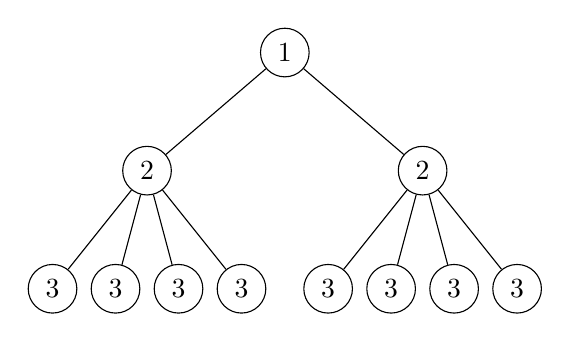
\begin{tikzpicture}[
            level 1/.style={sibling distance=35mm},
            level 2/.style={sibling distance=8mm},
          every node/.style = {shape=circle, rounded corners,
            draw, align=center,
            top color=white, bottom color=white}]]
          \node {1}
            child { node {2} 
                child { node {3} }
                child { node {3} }
                child { node {3} }
                child { node {3} } } 
            child { node {2}
                child { node {3} }
                child { node {3} }
                child { node {3} }
                child { node {3} } };
        \end{tikzpicture}   
    \caption{\acrshort{per} Sum Tree}
    \label{fig:sum_tree}
\end{figure}
Despite the distribution being skewed in favour of sampling experiences that yielded higher rewards, all experiences still have a non-zero chance of being sampled from the \acrshort{per}, ensuring that the \acrshort{drl} is not outright discounting any experiences. 
The stochastic sampling method in use with the \acrshort{per} is shown in \ref{eq:stochastic_per_sampling} \cite{schaul_prioritized_2016}.
\begin{equation} \label{eq:stochastic_per_sampling}
   P(i) = \frac{p_{i}^{\alpha}}{\sum_{k}^{K} p_{k}^{\alpha}} , \ p^{\alpha} > 0
\end{equation}
In \ref{eq:stochastic_per_sampling}, $p_{\alpha}$ is the priority of transition $i$. 
The exponent $\alpha$ determines how much prioritisation is used, with $\alpha = 0$ being the uniform sampling case. 
As the distribution is being changed based on the priority of a given state-wise transition and the system is reliant on expectation value of the update being the same as the expectation of its estimated value, bias is introduced to the sampling and must be corrected for. 
The bias is corrected for using \acrfull{is} weights, shown in \ref{eq:importance_sampling_weight}. 
The \acrshort{is} weights fully compensate for the non-uniform sampling probabilities when $\beta = 1$ \cite{schaul_prioritized_2016}. 
\begin{equation} \label{eq:importance_sampling_weight}
   w_{i} = \begin{pmatrix}
       \frac{1}{N} \frac{1}{P_{i}}
   \end{pmatrix}^{\beta}
\end{equation}
\subsection{\texorpdfstring{\acrshort{ans}}{ANS} Generation for Eavesdropping Links}
For a set of $\mathcal{M}$ Eves attempting to perform \acrshort{mitm} attacks on the set of $\mathcal{K}$ \acrshort{lu}s, the \acrshort{uav}-\acrshort{bs} must dynamically adjust a noise signature for the legitimate \acrshort{gu}s to filter out to maximise the secrecy rate. 
This is done to minimise the eavesdropping rate and in turn, maximise the secrecy rate. 
To achieve this, the \acrshort{uav}-\acrshort{bs} introduces an \acrshort{ans} to the signals being transmitted and received in the \acrshort{lu} communications channels based on the worst-case estimate of the eavesdropping rate. 
The \acrshort{ans} is generated by the \acrshort{uav}-\acrshort{bs}, which observes the position of all of the non-authenticated \acrshort{gu}s and calculates the evesdropping rate for all of the perceived Eves for each \acrshort{lu}. 
A scaling variable, $\rho$ is calculated to amplify the noise signature $\psi$ based on the proximity of any given Eve to each \acrshort{lu}. 
For greater levels of proximity of an Eve, measured by $d_{E, k}$ relative to the maximum flight zone distance, the value of $\rho$ increases, as shown in \ref{eq:rho_ans_scaling_variable}. 
\begin{equation} \label{eq:rho_ans_scaling_variable}
   \rho = \begin{bmatrix}
       \frac{d_{max, k} - d_{E, k}}{d_{max, k}}
   \end{bmatrix} ^{-1}
\end{equation}
This variable is then used to scale the \acrshort{ans} waveform as shown in \ref{eq:ans_waveform}. 
\begin{equation} \label{eq:ans_waveform}
   \psi = \rho P_{U, k}^{Tx} \cos(f_{n})
\end{equation}
Where $f_{n}$ is the frequency of the \acrshort{ans} waveform, which is also scaled by $\rho$ as shown in \ref{eq:ans_frequency}.
\begin{equation} \label{eq:ans_frequency}
   f_{n} = \rho f_{c}
\end{equation}
\section{Software Engineering \& Implementation}
The simulation was written in the Python programming language and structured using the \acrfull{oop} programming paradigm.
All code and scripts in use for the project besides the \acrshort{per} implementation were written from scratch. 
The key packages that were used to design the simulation were OpenAI's Gymnasium and PennyLane frameworks, made for deep reinforcement learning and quantum machine learning applications, respectively. 

Git was used for software version control throughout the entire development of the project. Different features were tested on their own branches and eventually merged into the main branch once they were functioning as intended. 

The initial experiments for testing particular features and ensuring that the code would run reliably were performed locally, however, as the computational load began to increase for longer and more comprehensive experiments, the Sonic \acrfull{hpc} cluster provided by the university was used with batch scripts, written in \acrshort{bash}, running the Python experiment script while writing the output log data to a text file for post-processing data analysis. 
\subsection{Custom Gymnasium Environment}
\acrshort{uav}s, \acrshort{gu}s and the Gymnasium environment are modelled as classes with particular attributes. 
Inheritance is utilised for different subclasses of \acrshort{gu}, i.e., \acrshort{lu}s and Eves and for different classes of \acrshort{uav}s so that the design is extensible to support different classes of \acrshort{uav}, such as \acrshort{uav} relays and separate \acrshort{uav}s for interfering with \acrshort{mitm} attacks from Eves. 

These classes were written to ensure that the design can be extended for other network architectures, however, in the final implementation, the \acrshort{uav}-\acrshort{bs} handles the \acrshort{ans} generation. 

All of the core computation involving the environment is contained within functions for computing $\eta_{EE} (t)$, the channel dynamics, \acrshort{ans} generation, reward allocation, \acrshort{uav} movement, subchannel allocation for \acrshort{lu}s and observation of the constraints is handled within the environment program. 

There are also functions for accessing the results of these calculations in getter methods so that the top-level script can access this data for logging and visualisation purposes. 
\subsection{Top-Level Program}
The overall simulation was designed with separate programs, each serving a particular purpose and all called upon using a top-level Python script in which the simulation parameters are instantiated, e.g., the capacity of the \acrfull{mer} or \acrfull{per} buffer, the number of layers in the actor-critic network ansatz, the number of episodes to be run, the \acrshort{mer} or \acrshort{per} random sampling batch size, target directories for the output data and the data visualisation.  

The actor and critic loss, gradient optimisation and gradient descent calculations are also handled in this script, where the computed quantum gradients are updated in the quantum circuitry. 
The gradients are computed using the JAX interface and the Optax library is in use for the optimisation of the gradients. 

The JAX interface was chosen for its \acrfull{jit} compilation via OpenXLA, open-source machine learning compiler ecosystem.
This script imports the custom Gymnasium environment, the \acrshort{mer}, the \acrshort{per} and the quantum circuits for the actor and critic network. 
\subsection{Simulated Quantum Circuits}
The quantum actor-critic network Python program contains the function definitions for the quantum circuits using the PennyLane library as well as the functions for visualisation the quantum circuits and the decoding operations for both the actor and critic networks. 
The critic class contains a method for evaluating the Q-value for the action taken by the actor, which is called for each timestep within the simulation.
The JAX interface is specified for the quantum circuits and the qubit type is the PennyLane lightning qubit, which is contained within the PennyLane-Lightning library for faster computation and has a C++ backend as opposed to a Python one. 
The decoded outputs are vectorised within the top-level experiment script using JAX's NumPy-like arrays. 
\section{Simulation Parameters \& Chosen Scenario}
The values that were used in the simulations are listed in Table \ref{table:simulation_values}.
These parameters were used to yield the results presented in the following chapter. 
The scenarios tested as part of this research did not involve obstacles within the flight zone.

\begin{table} [ht!]
    \centering
    %\begin{tabular}{ | m{3cm} | m{3cm} | m{3cm} | } 
    \begin{tabular}{ | c | c | c | } 
         \hline
         \textbf{Parameter} & \textbf{Definition} & \textbf{Value} \\ [0.75ex] 
         %\hline\hline
         \hline
         Ep & Number of Episodes & 30 \\ 
         \hline
         B & \acrshort{per} Sampling Batch Size & 30 \\
         \hline
         M & Number of Layers & 1-5 \\
         \hline
         $BW_{f_{c}}$ & Bandwidth & 1 MHz \\
         \hline
         K & Number of \acrshort{lu}s & 4 \\
         \hline
         E & Number of Eves & 2 \\  
         \hline
         X & Number of \acrshort{uav}-\acrshort{bs}s & 1 \\
         \hline
         $\sigma_{\acrshort{los}}^{2}$ & \acrshort{los} Noise & -100 dBm \\ 
         \hline
         $\sigma_{\acrshort{nlos}}^{2}$ & \acrshort{los} Noise & -80 dBm \\ 
         \hline
         $R_{min}$ & Minimum Data Rate & 9.5 Mbps \\
         \hline
         $R_{min}^{sec}$ & Minimum Secrecy Rate  & 9.5 Mbps \\
         \hline
         $x_{max}, y_{max}, z_{max}$ & Flight Area & 150 m, 150 m, 122 m \\ 
         \hline
         $x_{min}, y_{min}, z_{min}$ & Minimum \acrshort{uav} Co-ordinates & 0 m, 0 m, 10 m \\ 
         \hline
         $\zeta$ & Air Density & 1.225 kg m$^{-3}$ \\
         \hline
         $\sum_{i=1}^{2} n_{i}$ & Mass of \acrshort{uav} Frame \& Battery & 1.46 kg \\ 
         \hline
         $\textbf{K}$ & Lift-to-Drag Ratio & 6.65 \\ 
         \hline
         $K_{shots}$ & Number of Quantum Measurements & 1024 \\
         \hline
         $\beta_{actor}$ & Actor Learning Rate & 0.01 \\
         \hline
         $\beta_{critic}$ & Critic Learning Rate & 0.01 \\
         \hline
         $V_{max}$ & Maximum \acrshort{uav} Velocity & 50 m s$^{-1}$ \\
         \hline
         $P_{U, max}^{Tx}$ & Maximum Transmit Power & 30 dBm \\
         \hline
         $A_{1}$, $A_{2}$ & Rician Channel Characteristics & 4, 0.1 \\
         \hline
         $E_{max}$ & Total \acrshort{uav} Energy & 50 kJ \\
         \hline
         r & Number of \acrshort{uav} Rotors & 4 \\
         \hline
         $\theta$ & Spinning Blade of 1 Rotor & 0.0507 m$^{2}$ \\
         \hline
         $\mu$ & Discount Factor & 0.99 \\
         \hline
    \end{tabular} 
    \caption{Simulation Parameters}
    \label{table:simulation_values}
\end{table}
Multiple \acrshort{uav}s were tested along with larger numbers of \acrshort{gu}s early in the development of this project, however, the problem was reduced to a single-agent \acrshort{drl} approach rather than immediately starting with a multi-agent reinforcement learning (\acrshort{marl}) approach. 
This is also a very computationally intensive system to simulate, so fewer of \acrshort{gu}s and a single \acrshort{uav}-\acrshort{bs} led to the simulations being faster and a greater ability to debug and improve the system throughout the development of the simulations. 
A classical \acrshort{drl} implementation was attempted early in the development of the project for comparative purposes, however, this proved to detract from the \acrshort{lqdrl} implementation and was abandoned. 